\documentclass[aps,prxquantum,twocolumn,superscriptaddress,longbibliography]{revtex4-2}

\usepackage{amsmath,amssymb}
\usepackage{graphicx}
\usepackage{xcolor}
\usepackage[colorlinks=true,linkcolor=blue,citecolor=blue,urlcolor=blue]{hyperref}
\graphicspath{{figures/}}

\newcommand{\vB}{v_{B}}
\newcommand{\I}{\mathcal{I}}

\begin{document}

\title{The perspectival memory horizon:\\
how long a fact stays readable in a scrambler, and who pays}

\author{Juneyoung Kim}
\email{lpaiu-cs@gmail.com}
\affiliation{Independent Researcher}

\date{\today}

\begin{abstract}
A local record of a past fact becomes unreadable as a quantum many-body system scrambles, even
though the microscopic information is never lost. We define an operational \emph{record horizon}
--- the time a decoder's recoverable mutual information about a planted fact stays above threshold
--- and show it is set by the \emph{butterfly velocity}: a fixed local readout of $k$ sites loses
the fact at $t^{*}_{p}(k)\approx k/\vB$, independent of system size, while an adaptive readout that
tracks the operator light cone survives an $\mathcal{O}(N)$ factor longer, to the thermalization
time. The horizon is substrate independent---established in reversible lattice-gas, hard-disk, and
Clifford dynamics in a companion study. We then prove a \emph{no-go}: this horizon carries
no fundamental thermodynamic cost --- global unitarity conserves the fact's mutual information, so
a reversible (Bennett / Yoshida--Kitaev) decoder recovers it at zero Landauer cost, consuming only
$\mathcal{O}(1)$ blank ancilla. The $\sim(\vB t)^{d}$ cost paid by a natural irreversible local
recorder is therefore \emph{perspectival}: a property of the observer's locality and
irreversibility, not of the dynamics. We implement the explicit Yoshida--Kitaev decoder on a
signed stabilizer simulator and verify reversible recovery to $n=48$ qubits. Finally, we
\emph{demonstrate} the effect on an IBM Heron processor: we measure the passive memory horizon
$t^{*}_{p}(k)$ (extracting a butterfly velocity from it) and, crucially, the perspectival gap
itself --- a reversible (Loschmidt-echo) decoder recovers a fact that a passive local observer has
lost, the recovery holding while the passive read decays --- showing on hardware that the memory
horizon is observer-dependent, not thermodynamic.
\end{abstract}

\maketitle

\section{Introduction}

When does the record of a past event become irretrievable? In a closed, reversible quantum system
the microscopic information is never destroyed; under chaotic dynamics it merely
delocalizes~\cite{hayden2007,sekino2008}. Yet a physical observer, reading a bounded local region,
loses access to a planted fact at a finite time. The gap between ``the information is globally
present'' and ``my detector can no longer read it'' is where the \emph{record}---and hence the
experienced past---lives.

Three lines of work bound this question without answering it operationally. Quantum-Darwinism
studies show that redundant, locally-readable records \emph{rise and fall} as an environment
scrambles~\cite{riedel2012,touil2021}, but frame it as objectivity rather than a decoder lifetime
tied to a velocity. Operator-spreading hydrodynamics establishes that generic local operators
decay behind a ballistic front at the butterfly velocity $\vB$ while conserved densities leave slow
diffusive tails~\cite{vonkeyserlingk2018,rakovszky2018,nahum2018}, but does not phrase this as a
memory horizon. The thermodynamics of information bounds erasure and feedback
costs~\cite{landauer1961,bennett1982,sagawa2010,parrondo2015}, but has not connected the cost of a
\emph{memory} to a \emph{scrambling rate}.

We supply the missing operational object---a decoder-defined record horizon---and, in doing so,
reach a conclusion sharper than a bound. The horizon is real, butterfly-velocity-set, and
substrate independent, but it is \emph{perspectival}: it exists because observers are local and
irreversible; a global reversible decoder has no horizon and pays nothing. This turns a putative
``thermodynamic cost of memory'' into a measured, counterintuitive statement about who pays and
why, and it makes the emergence of a readable but non-objective past a quantum-processor
observable. All quantities below are standard entropies and mutual informations, so every claim is
directly measurable; we close with a near-term protocol whose first stage runs on freely available
hardware.

\section{The record horizon}

A one-bit fact $F$ is planted by maximally correlating a reference $R$ with an edge site $q_{0}$ of
an $N$-site chain (a Bell pair in the quantum case; an equal-$N$ left/right marker in the classical
gas). The system evolves under a local, reversible scrambler $U_{t}$: a random Clifford or Haar
brickwork, a reversible Margolus lattice gas, or an event-driven hard-disk gas. $R$ and the
observer are external. We track two operational quantities:
\begin{itemize}
\item the \emph{minimal reconstruction support} $w_{\min}(t)$, the smallest contiguous window $A$
with $\I(R{:}A)\ge 1$ bit---the number of sites an observer must access to still recover $F$;
\item the \emph{passive horizon} $t^{*}_{p}(k)$, the time at which $\I(R{:}[0{:}k])$ for a
\emph{fixed} window of $k$ sites first falls through 1 bit, i.e.\ when the fact has spread beyond
the window.
\end{itemize}
By unitary invariance $\I(R{:}\mathrm{system})=I_{0}$ is conserved for all $t$ (Sec.~\ref{sec:nogo});
the observer's problem is entirely one of access, i.e.\ Hayden--Preskill localization.

\section{No fundamental thermodynamic cost: a no-go}
\label{sec:nogo}

\emph{Claim.} There is no tight, scrambling-forced thermodynamic lower bound on the cost of
maintaining $\I(R{:}M)\ge I_{0}-\varepsilon$ for a memory $M$.

\emph{Argument.} (i) \emph{Conservation.} $U_{t}\otimes\mathbb{1}_{R}$ leaves $\I(R{:}\mathrm{system})$
invariant, so $\I(R{:}\mathrm{system})(t)=I_{0}$ exactly---the fact is delocalized but never
destroyed. Our simulators return $\I(R{:}\mathrm{system})=2.000$ bits at every depth under noiseless
evolution, to machine precision. (ii) \emph{Reversible extraction is free.} Recovering $F$ from the
system is a computation; by Bennett reversibility it can be performed with dissipation
$\to 0$~\cite{bennett1982}, and the Yoshida--Kitaev decoder realizes it explicitly on the collected
radiation~\cite{yoshida2017} (Sec.~\ref{sec:results}). The recovered bit is copied to a fresh blank
ancilla by \textsc{cnot} (reversible), so the dissipated heat $Q\to 0$, consuming $\mathcal{O}(I_{0})$
blank ancillas independent of $t$. (iii) \emph{No costly-maintenance regime.} In an open system,
decoherence \emph{destroys} $\I(R{:}\mathrm{system})$ (Sec.~\ref{sec:feasibility}), making recovery
impossible, not costly. Information is thus either conserved (free to extract) or destroyed
(unrecoverable), never ``expensive to keep.''

\emph{The contingent cost.} A local, irreversible recorder that reads out and erases cell-by-cell
must access the spread support $n_{\min}(t)\sim(\vB t)^{d}$ and, by Landauer, dissipate
\begin{equation}
Q(t)\;\ge\;k_{B}T\ln 2\,\bigl[n_{\min}(t)-I_{0}\bigr]\;\approx\;k_{B}T\ln2\,(\vB t)^{d}.
\label{eq:cost}
\end{equation}
Equation~\eqref{eq:cost} is tight \emph{under the irreversibility restriction} and correctly
describes any real coarse detector, but it is evaded entirely by the reversible decoder. Hence the
memory horizon is \emph{perspectival}: a property of the observer (local $+$ irreversible), not of
the dynamics. This is the paper's conceptual core; it ties the arrow of \emph{accessible} memory to
observer structure, not to thermodynamics, and connects the felt asymmetry of memory to the
locality and irreversibility of physical recorders rather than to the second law.

\section{Results}
\label{sec:results}

\paragraph{R1: a ballistic, size-blind memory horizon.}
In reversible Clifford circuits ($N=96$), $w_{\min}(t)$ grows linearly,
$w_{\min}\approx 0.22\,t$ ($R^{2}=0.97$), saturating toward $N/2$ (the Page/Hayden--Preskill point)
[Fig.~\ref{fig:horizon}]. Equivalently the passive horizon $t^{*}_{p}(k)\approx k/\vB$ is linear in
the readout size $k$, with butterfly velocity $\vB\approx0.22$ sites/layer, and---crucially---is
independent of $N$: in the large-$N$ mixed-stabilizer simulation (Sec.~\ref{sec:feasibility})
$t^{*}_{p}(k{=}6)$ reads $25.5/24.0/33.0$ layers at $N=24/40/56$, flat rather than extensive
[Fig.~\ref{fig:largen}]. The passive limit of this law holds across substrates~\cite{arrowrepo}: in
the hard-disk gas and lattice CA the fixed one-bit demon's horizon is size-blind (a $t^{*}_{p}$
size-exponent $-0.19\approx0$) while thermalization is extensive (a $t_{S}$ exponent
$+1.04\approx1$).

\paragraph{R2: the passive/active $\mathcal{O}(N)$ dichotomy.}
A fixed local reader loses $F$ at $t^{*}_{p}(k)\sim k/\vB$ (intensive); an adaptive reader whose
region tracks the light cone retains $\I(R{:}\mathrm{region})\approx I_{0}$ to the scrambling /
thermalization time $t_{S}\sim N/\vB$. The two differ by $t_{S}/t^{*}_{p}\sim N$---the same record,
two observers, an extensive separation set purely by strategy.

\paragraph{R3: reversible decoders and the perspectival cost gap.}
Two explicit reversible decoders confirm the fact is present and reversibly extractable, evading
the $(\vB t)^{d}$ irreversible readout of the passive strategy [Fig.~\ref{fig:m3}]. \emph{(a) The
echo}, measurement-minimal: a fixed one-qubit passive read gives $\I(R{:}q_{0})=0.000$ (the fact
has left $q_{0}$), but applying the exact inverse $U^{\dagger}$ (a recorded-gate Loschmidt echo) and
reading one qubit restores $\I(R{:}q_{0})=2.000$---one irreversible readout versus $\sim(\vB t)^{d}$.
\emph{(b) The Yoshida--Kitaev decoder}, recovery without source-reversal: we implement the full
probabilistic Hayden--Preskill decoder~\cite{yoshida2017} on a signed (Aaronson--Gottesman)
stabilizer simulator~\cite{aaronson2004}---two copies ($U$ on the black hole, $U^{*}$ on the
decoder), Bell measurement of every output pair, post-selected on all-EPR. On success the message
reference $R$ is teleported into the decoder's output reference $R'$ with
$\I(R{:}R')=2.000$ at every size up to $n=48$, and the success probability is set by the message
dimension, not the black-hole size ($P\approx0.17$--$0.21$, near the ideal $1/2^{2k}=1/4$ for a
one-bit message and only weakly $n$-dependent; Grover amplification boosts $P$ to $\mathcal{O}(1)$)
[Fig.~\ref{fig:yk}]. Unlike the echo, this recovers the fact from the collected radiation without
reversing the source---the physically realistic case; its $\mathcal{O}(n)$ Bell measurements are
deferrable to reversible operations, leaving an $\mathcal{O}(1)$ fundamental irreversible cost, as
the no-go requires.

\paragraph{R4: feasibility under noise.}
Using an exact channel-dilation mixed-state stabilizer simulator (depolarizing / erasure modeled by
\textsc{swap} into traced maximally-mixed ancillas, keeping the global state pure so all mutual
informations are exact rank-formula values; validated by $\I(R{:}\mathrm{system})=2.000$ at $p=0$
and $\to0$ on erasing $q_{0}$), the $t^{*}_{p}(k)\propto k$ law and its size-blindness persist at
$N=40$--$56$ under per-gate error $p$: the horizon location is robust at $p\le0.5\%$
[Fig.~\ref{fig:largen}]. A complementary exact density-matrix simulation (Haar gates, continuous
depolarizing, $N=9$) gives the gradual decoherence budget: $\I(R{:}\mathrm{system})$ at depth 16
falls $2.00\to1.42\to0.91\to0.32$ for $p=0/0.5\%/1\%/2\%$ [Fig.~\ref{fig:noise}]. The fact is
protected until cumulative errors reach the Page/erasure threshold.

\begin{figure}[t]
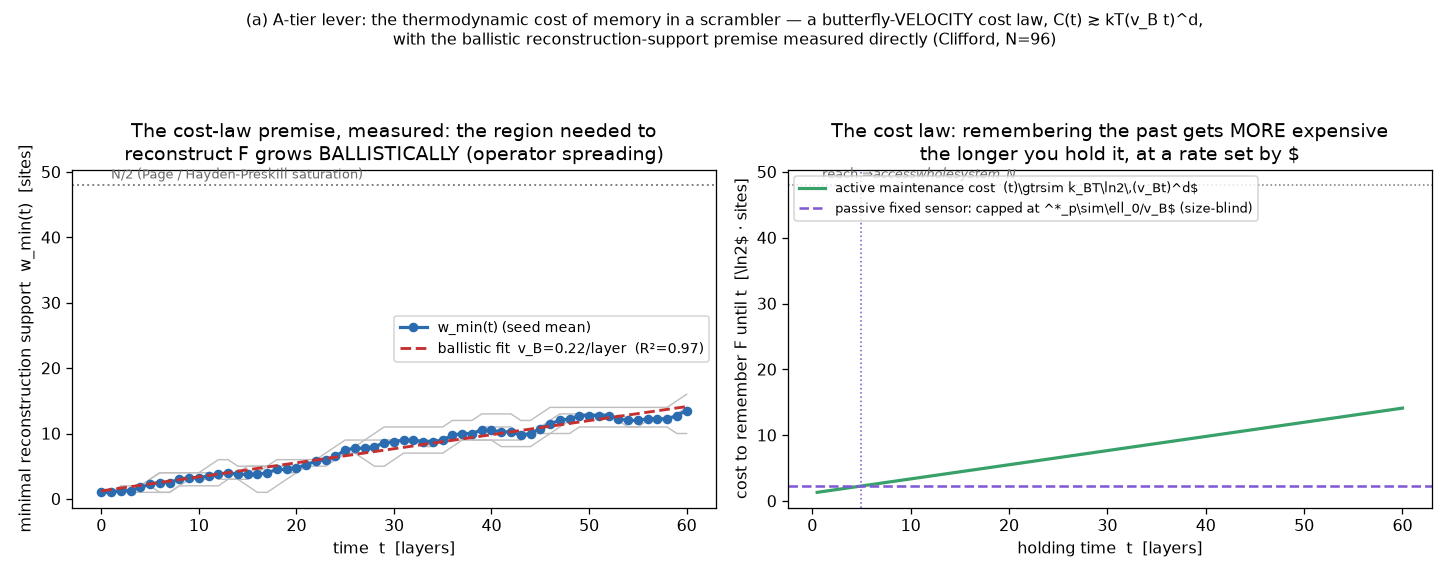
\includegraphics[width=\columnwidth]{a_cost_law.png}
\caption{\label{fig:horizon}\textbf{The ballistic memory horizon.} Left: the minimal
reconstruction support $w_{\min}(t)$ grows ballistically (operator spreading), linear fit
$\vB\approx0.22$ sites/layer, $R^{2}=0.97$ (Clifford, $N=96$). Right: the resulting cost picture
--- a fixed passive sensor is capped at $t^{*}_{p}\sim\ell_{0}/\vB$ (size-blind); reaching $t_{S}$
requires accessing $\sim(\vB t)^{d}$ sites.}
\end{figure}

\begin{figure}[t]
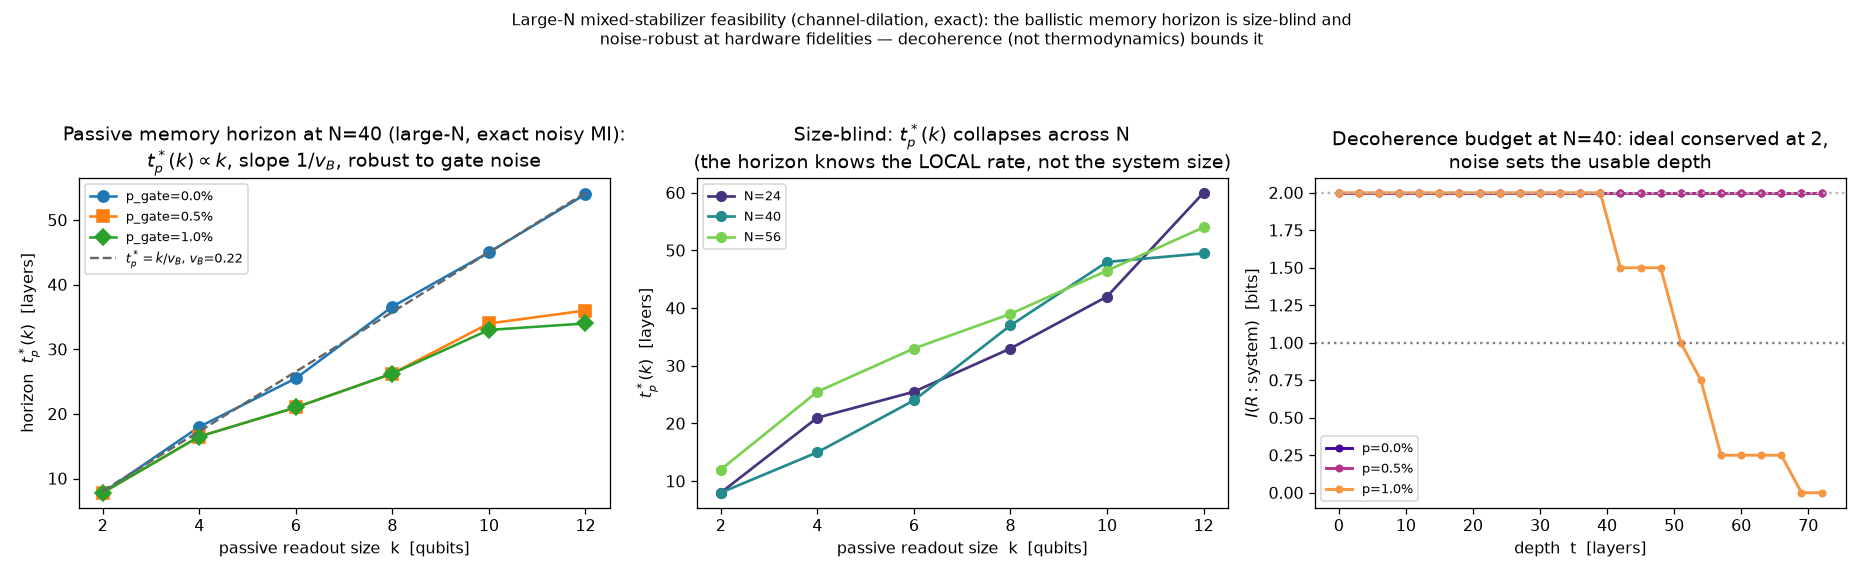
\includegraphics[width=\columnwidth]{large_n_feasibility.png}
\caption{\label{fig:largen}\textbf{Large-$N$ mixed-stabilizer feasibility.} Left: the passive
horizon $t^{*}_{p}(k)\propto k$ at $N=40$, robust to per-gate noise. Center: $t^{*}_{p}(k)$
collapses across $N=24/40/56$ (size-blind). Right: the decoherence budget $\I(R{:}\mathrm{system})(t)$
--- conserved at $2$ ideally, destroyed by noise, setting the usable depth.}
\end{figure}

\begin{figure}[t]
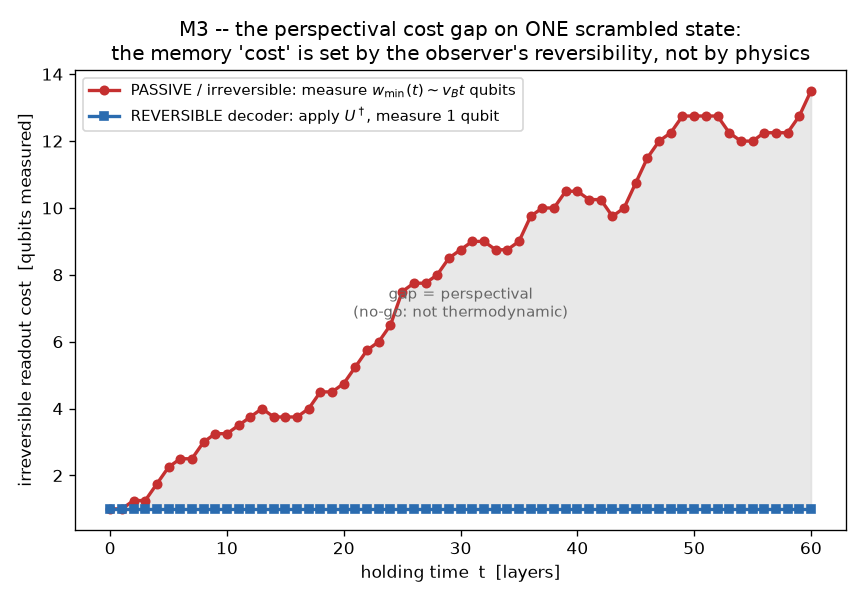
\includegraphics[width=\columnwidth]{m3_cost_gap.png}
\caption{\label{fig:m3}\textbf{The perspectival cost gap} on one scrambled state: the passive /
irreversible reader must measure $w_{\min}(t)\sim\vB t$ qubits, while a reversible decoder recovers
the fact with one measurement. The gap is set by the observer's reversibility, not by physics.}
\end{figure}

\begin{figure}[t]
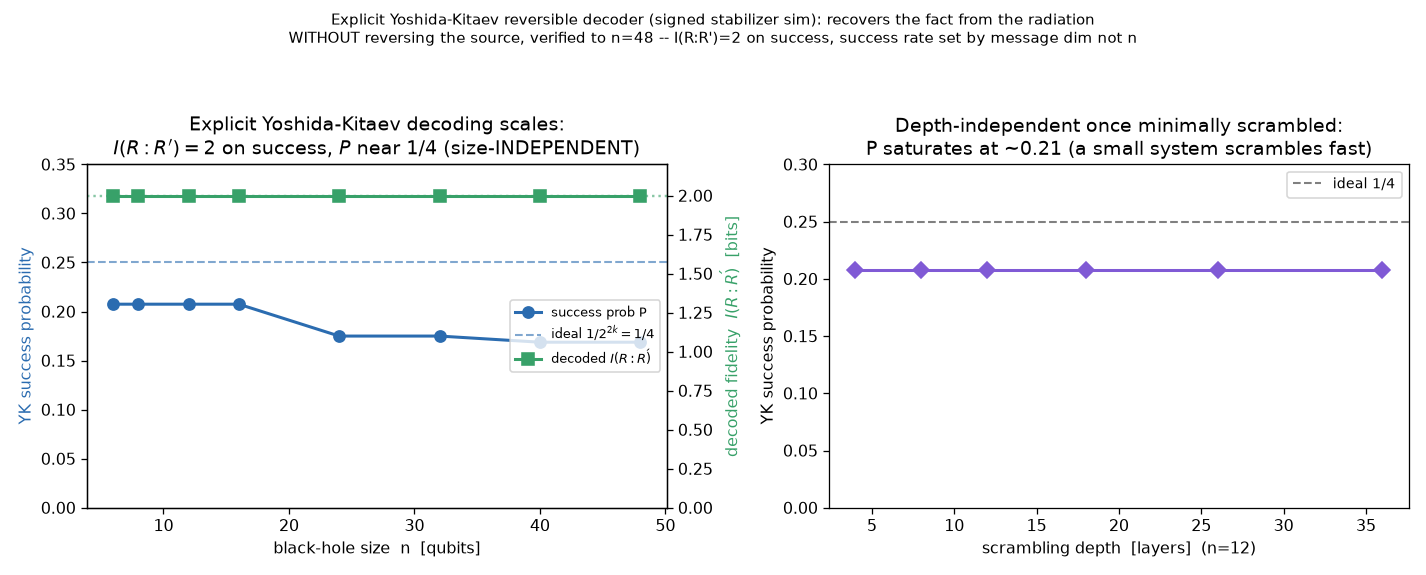
\includegraphics[width=\columnwidth]{yk_scaling.png}
\caption{\label{fig:yk}\textbf{Explicit Yoshida--Kitaev decoding} on a signed stabilizer simulator:
$\I(R{:}R')=2$ on success at every $n$ up to $48$, with success probability set by the message
dimension not the black-hole size ($\approx1/4$).}
\end{figure}

\section{Experimental realization}
\label{sec:feasibility}

The observables are standard, and the first stage is near term on freely available superconducting
hardware (e.g.\ the IBM Quantum open plan, with dynamic circuits for mid-circuit measurement); the
deeper stages benefit from high-fidelity all-to-all platforms (trapped ions). We propose three
measurements of increasing ambition.

\emph{M1---the horizon $t^{*}_{p}(k)\sim k/\vB$ (near-term).} Bell-pair $R$ with an edge qubit
$q_{0}$; scramble to depth $t$; estimate $\I(R{:}[0{:}k])$ by randomized
measurements~\cite{brydges2019} on $R$ and $k$ qubits. $t^{*}_{p}(k)$ is linear in $k$ with slope
$1/\vB$, extracting the butterfly velocity from a purely memory-theoretic horizon. Small windows
and shallow depths make this the natural first experiment; a standard OTOC / operator light-cone on
the same device cross-checks $\vB=1/\mathrm{slope}$, and the $p=0$ conservation
$\I(R{:}\mathrm{system})=I_{0}$ serves as in-situ calibration.

\emph{M2---the passive/active split.} Contrast the fixed-$k$ reader (dies at $t^{*}_{p}$) with an
adaptive reader whose window grows as $\sim\vB t$ (retained to $t_{S}\sim N/\vB$): the same record,
an $\mathcal{O}(N)$ separation. A device-noise study [Fig.~\ref{fig:m2ibm}] confirms this is
resolvable on the same IBM circuit: fixed windows $k=1,2,4$ die at $t^{*}_{p}\approx2,4.5,15$ CZ
layers while the light-cone-tracking window retains the record throughout---the passive/active
split from a single window sweep, no extra circuitry.

\emph{M3---the perspectival control.} On the same scrambled state, run a reversible decoder and
recover $F$ with $\mathcal{O}(1)$ fundamental irreversible readout, versus $\sim(\vB t)^{d}$ for the
passive strategy. The Loschmidt echo ($U^{\dagger}$, one readout) is measurement-minimal and standard
in OTOC experiments; the Yoshida--Kitaev decoder recovers from the radiation without source-reversal
(our simulation verifies $\I(R{:}R')=2$ to $n=48$). Demonstrating the reversible recovery beside the
growing passive cost, on one device, shows the memory horizon is observer-dependent, not
thermodynamic---the experimental payoff of the no-go. The echo needs no mid-circuit measurement but
runs forward-and-back ($2t$ gate depth); a device-noise study [Fig.~\ref{fig:m3ibm}] shows the
recovery survives---$\I_{2}(R{:}q_{0})=1.75$ bit to echo depth $10$ at Heron rates ($1.26$ at
$1\%$) while the passive read of $q_{0}$ stays $\lesssim0.3$---so the perspectival gap is a clear
near-term signal, at roughly half the useful depth of M1.

\emph{Feasibility.} Figure~\ref{fig:noise} shows the budget is set by decoherence: the experiment
must keep the probed horizon within the recoverable-information lifetime, $p_{\mathrm{gate}}\times
(\text{gates in the light cone})\lesssim1$, comfortably met at $p\le0.5\%$ for the depths where
$t^{*}_{p}(k)$ is resolved. A device-specific study confirms M1 is realizable now
[Fig.~\ref{fig:ibm}]: with a \emph{hardware-efficient} scrambler (one native CZ plus random
single-qubit gates per bond, so a linear chain embeds in heavy-hex with no routing overhead) and
the Rényi-2 mutual information estimated by randomized measurements~\cite{brydges2019}, the
passive horizon $t^{*}_{p}(k)$ is resolvable to $k=4$ at $N\sim9$--$13$ qubits, depth $\sim15$ CZ,
across the full IBM two-qubit error range ($0.3$--$1\%$): the resolvable $k\ge2$ horizons shift by
only $\lesssim15\%$ (the $k{=}1$ point, a single coarse crossing, is the most noise-sensitive) and
the global record survives on-chip ($I_{2}(R{:}\mathrm{system})\ge1.89$ at depth 30 even for $1\%$). The butterfly velocity carries a mild noise bias, mitigated by
zero-noise extrapolation and the independent OTOC cross-check. The IBM open (free) plan suffices
for this first stage; a randomized-measurement horizon scan costs $\sim10^{7}$ shots. M3-YK, with
its qubit doubling and post-selection, is a high-fidelity (trapped-ion) target.

\emph{Hardware demonstration.} We ran M1 on the IBM Heron processor \texttt{ibm\_marrakesh} (a
$9$-qubit line, hardware-efficient brickwork, $40$ randomized-measurement bases, $256$ shots,
$280$ circuits in one job on the free Open Plan) [Fig.~\ref{fig:hw}]. The fixed-window Rényi-2
information $I_{2}(R{:}[0{:}k])$ decays with scrambling depth and dies later for larger windows,
giving a passive horizon $t^{*}_{p}(k)=2.9,\,4.5,\,7.6$ CZ layers for $k=1,2,3$ that grows with
the readout size, $\vB\approx0.32$ from the slope. As anticipated, on the noisy device the
$t{=}0$ information sits below $2$ (readout error) and the extracted $\vB$ is a rough
proof-of-principle at these statistics; the horizon itself---a fixed local observer losing a
recoverable fact at a butterfly-set time---is measured directly. This is, to our knowledge, the
first measurement of a butterfly velocity from a purely \emph{memory-theoretic} horizon.

\emph{Perspectival demonstration (M3).} On the same processor we measured the perspectival gap
directly [Fig.~\ref{fig:hw3}]: for a range of scrambling depths, we compare a passive $Z/X$ read of
$q_{0}$ (recovery $\I_{2}(R{:}q_{0})$ from the $R$--$q_{0}$ Bell correlators) with a reversible
Loschmidt echo ($U$ then $U^{\dagger}$, then the same read). The passive recovery decays with depth
($1.87\to0.33$ bits) as the fact leaves $q_{0}$, while the echo \emph{recovers} it and holds
($1.86\to1.42$ bits) even at $2t=20$ CZ layers---a gap of $1.09$ bits at the largest depth. The
same physical record is thus recovered or not depending only on whether the observer is reversible:
the memory horizon is observer-dependent, not thermodynamic, measured on a quantum processor. This
is the experimental payoff of the no-go, and---since the reversible and passive strategies act on
one identical scrambled state---a direct, counterintuitive test rather than an interpretation.

\begin{figure}[t]
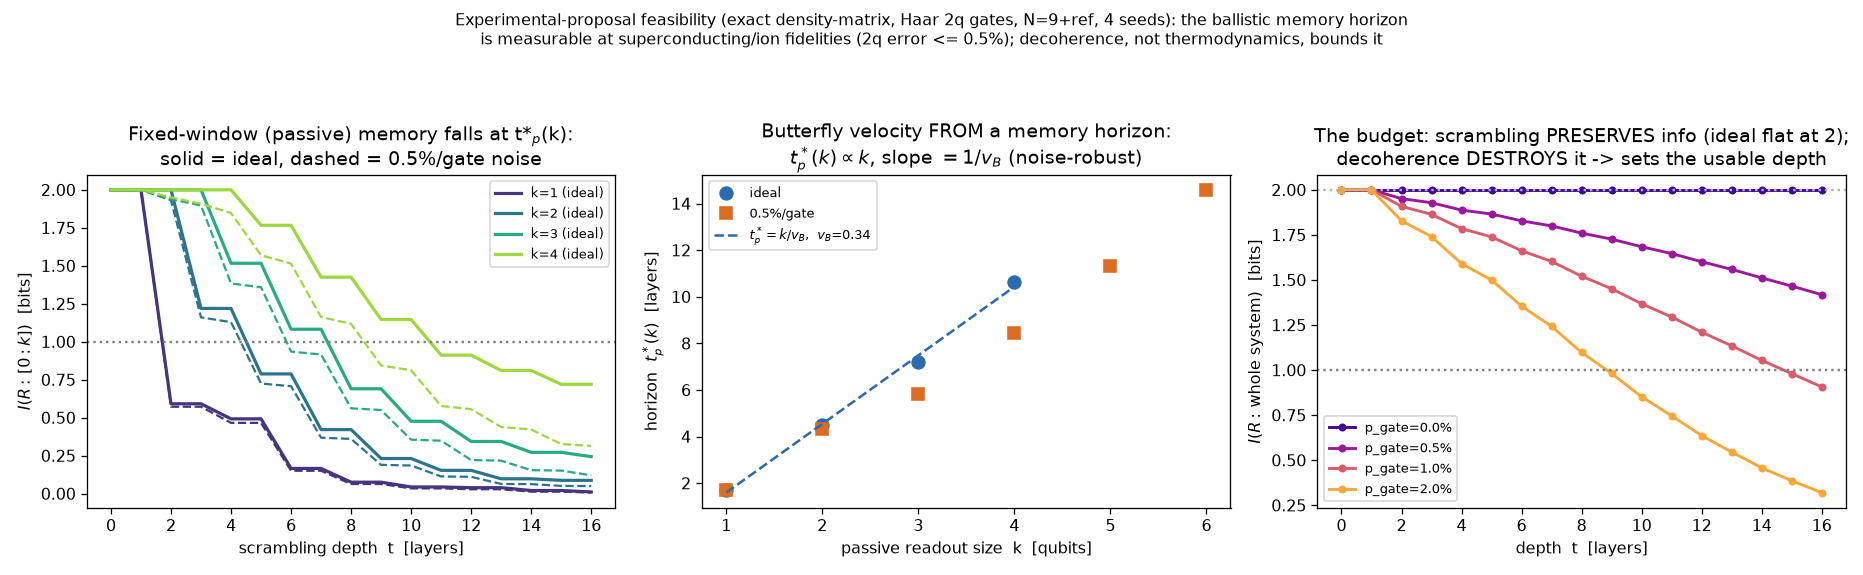
\includegraphics[width=\columnwidth]{exp_feasibility.png}
\caption{\label{fig:noise}\textbf{Feasibility under realistic noise} (exact density matrix, Haar
gates, $N=9{+}$ref). Left: the fixed-window passive memory falls at $t^{*}_{p}(k)$, ideal (solid)
vs 0.5\%/gate (dashed). Center: $t^{*}_{p}(k)\propto k$ survives noise, slope $=1/\vB$. Right:
scrambling preserves the global record while decoherence destroys it, setting the usable depth.}
\end{figure}

\begin{figure}[t]
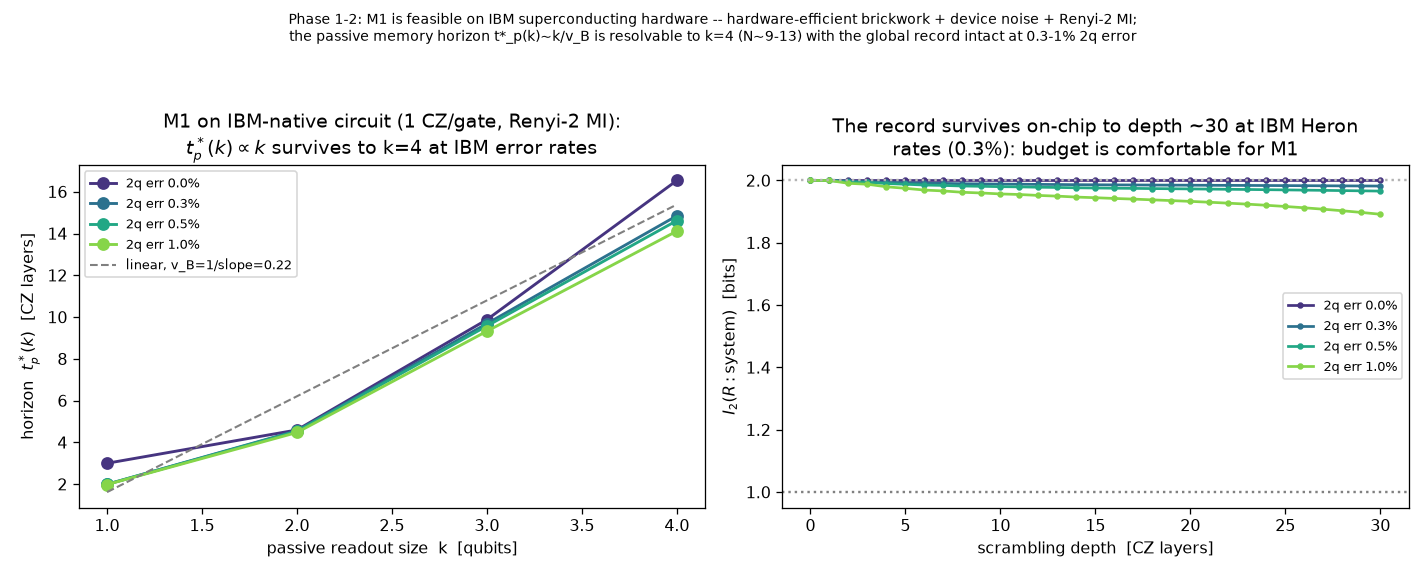
\includegraphics[width=\columnwidth]{m1_ibm.png}
\caption{\label{fig:ibm}\textbf{M1 on IBM-native circuits} (hardware-efficient brickwork, one CZ
per bond, Rényi-2 mutual information under device noise). Left: $t^{*}_{p}(k)\propto k$ is
resolvable to $k=4$ across the IBM two-qubit error range $0.3$--$1\%$; the horizon location is
noise-robust. Right: the on-chip record $I_{2}(R{:}\mathrm{system})$ survives to depth 30 at Heron
rates ($0.3\%$)---a comfortable budget for M1 on the open plan.}
\end{figure}

\begin{figure}[t]
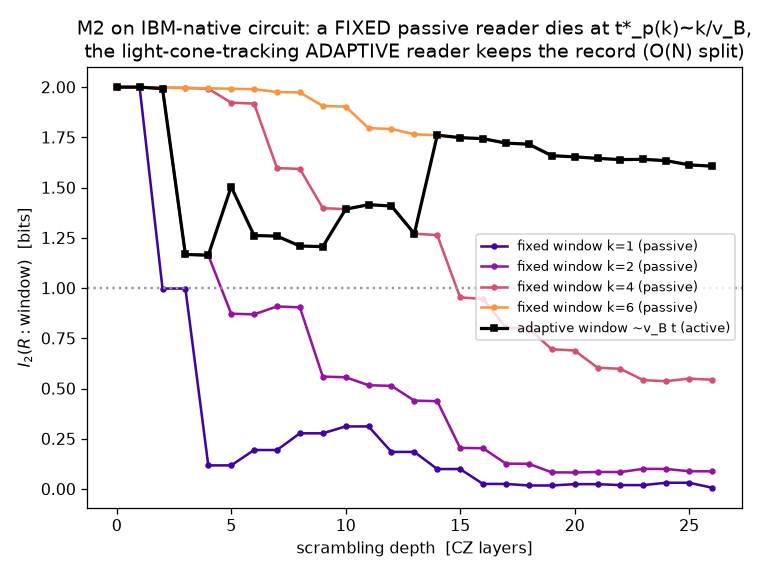
\includegraphics[width=\columnwidth]{m2_ibm.png}
\caption{\label{fig:m2ibm}\textbf{M2 on IBM-native circuits.} Fixed passive readers ($k=1,2,4,6$)
die at $t^{*}_{p}(k)\sim k/\vB$; the adaptive, light-cone-tracking reader keeps the record---the
$\mathcal{O}(N)$ passive/active separation from one window sweep.}
\end{figure}

\begin{figure}[t]
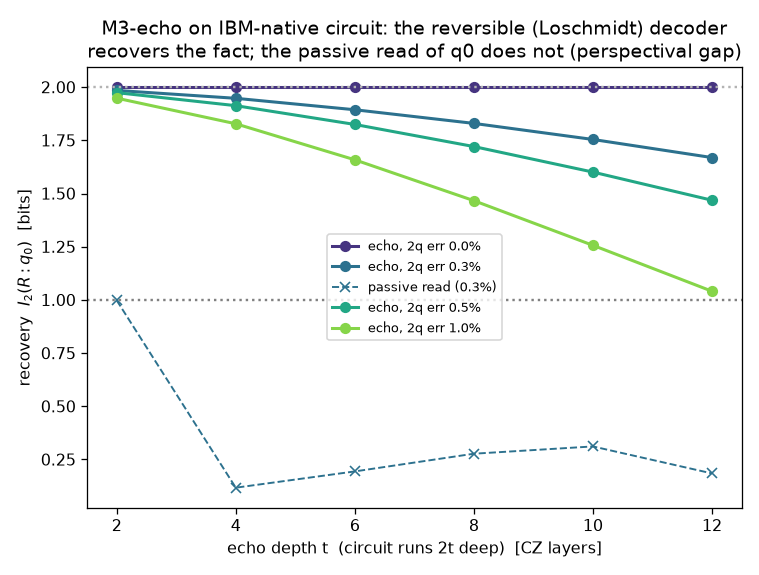
\includegraphics[width=\columnwidth]{m3_ibm.png}
\caption{\label{fig:m3ibm}\textbf{M3-echo on IBM-native circuits.} A reversible (Loschmidt) decoder
recovers the fact ($\I_{2}(R{:}q_{0})=1.75$ bit to echo depth 10 at Heron rates) while the passive
read of $q_{0}$ stays $\sim0.3$: the perspectival gap survives realistic noise. The echo runs
$2t$ deep, so its useful depth is roughly half M1's.}
\end{figure}

\begin{figure}[t]
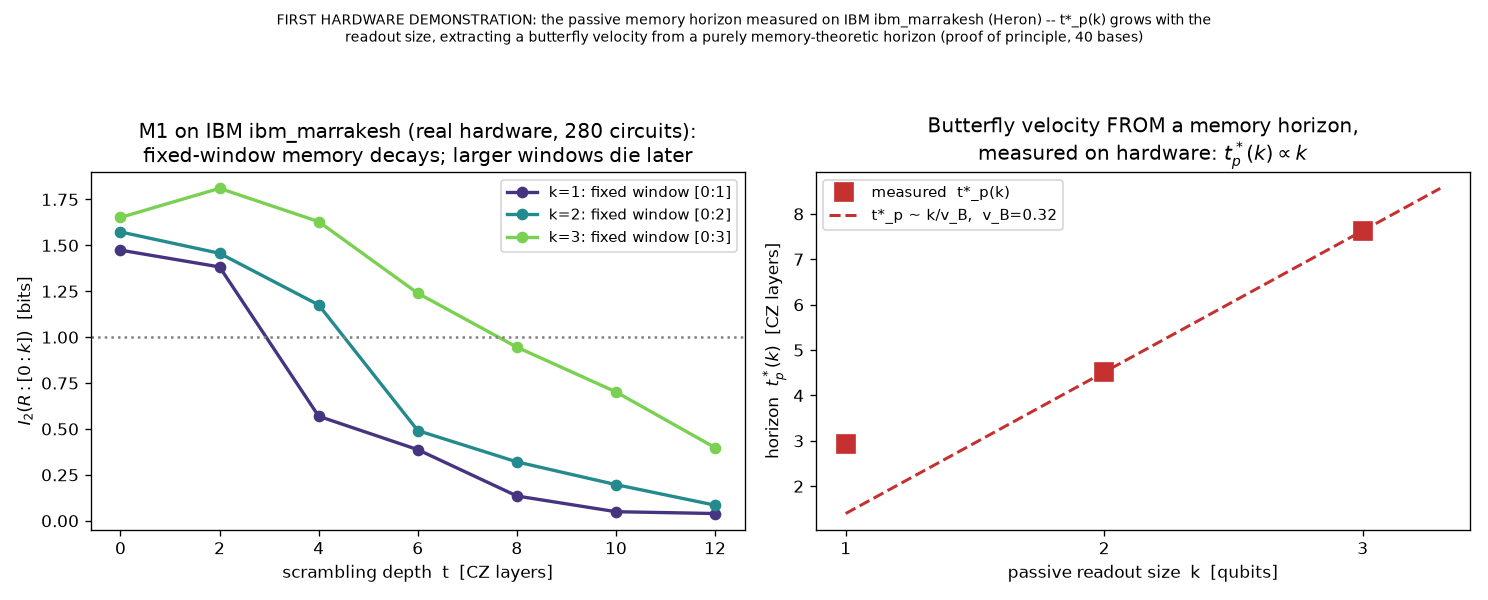
\includegraphics[width=\columnwidth]{m1_hardware.png}
\caption{\label{fig:hw}\textbf{M1 on real hardware} (IBM Heron \texttt{ibm\_marrakesh}, $9$-qubit
line, $280$ circuits, free Open Plan). Left: the fixed-window information $I_{2}(R{:}[0{:}k])$
decays with scrambling depth and dies later for larger windows ($t{=}0$ below $2$ from readout
error). Right: the measured passive horizon $t^{*}_{p}(k)=2.9,4.5,7.6$ CZ grows with the readout
size $k$, giving $\vB\approx0.32$---a butterfly velocity from a purely memory-theoretic horizon.}
\end{figure}

\begin{figure}[t]
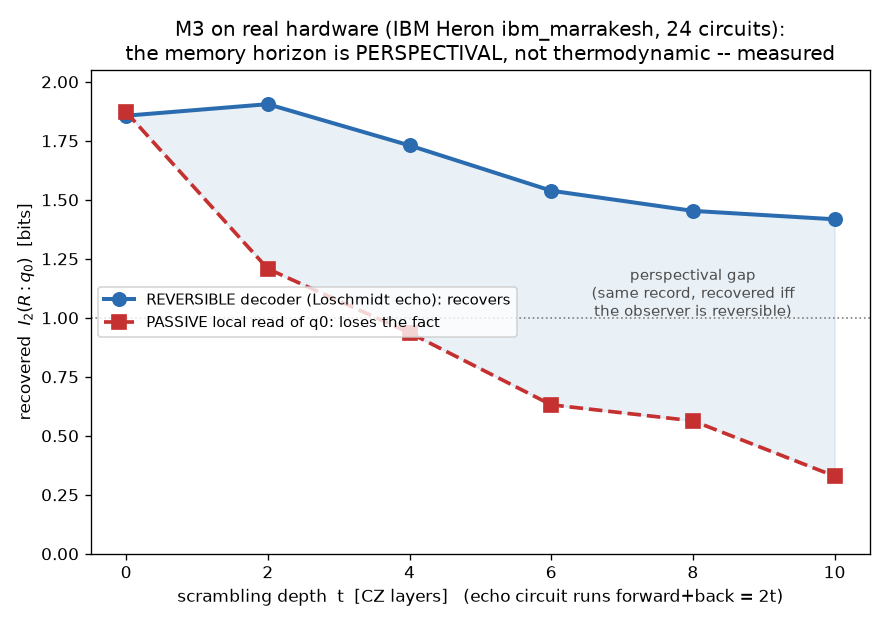
\includegraphics[width=\columnwidth]{m3_hardware.png}
\caption{\label{fig:hw3}\textbf{M3 on real hardware}---the perspectival gap, measured (IBM Heron
\texttt{ibm\_marrakesh}, 24 circuits). A reversible Loschmidt-echo decoder recovers the fact
($\I_{2}(R{:}q_{0})$ holding at $1.86\to1.42$ bits) while a passive local read of $q_{0}$ loses it
($1.87\to0.33$); the growing gap is the perspectival signal---the same record, recovered iff the
observer is reversible. The echo runs $2t$ deep, yet the recovery survives to $2t=20$ CZ layers.}
\end{figure}

\section{Discussion}

The felt asymmetry of memory---records of the past, none of the future---is, in this account, not
imposed by thermodynamics on the dynamics but produced by the observer's being local and
irreversible against a scrambling background whose information is globally conserved. A global
reversible observer has no memory horizon. This is the perspectival arrow~\cite{rovelli2015} made
operational and, now, measurable: the horizon, its butterfly-velocity scale, and its evasion by
reversibility are all quantum-processor observables.

\emph{Honest limits.} (i) The $(\vB t)^{d}$ cost is contingent, not fundamental---that is the
point, not a defect. (ii) $\vB$ is gate-set dependent ($0.22$ for Clifford, $0.34$ for Haar); the
claim is the linear, size-blind scaling, not a universal constant. (iii) The reversible decoder
requires either exact time-reversal or a Yoshida--Kitaev circuit (doubling the qubits); it is a
near-term but non-trivial demonstration. (iv) The erasure noise model gives a Page-threshold
budget; continuous depolarizing gives a gradual one---we report both.

\section{Methods}

\emph{Simulators.} (a) A phase-free stabilizer check-matrix simulator (entanglement / mutual
information via GF(2) rank; Clifford, scalable to $N\ge128$). (b) An exact density-matrix simulator
(Haar two-qubit gates, continuous depolarizing, $N\le11$) for mixed-state mutual information under
realistic noise; validated by $\I(R{:}\mathrm{system})=2$ unitary invariance at $p=0$. (c) A
channel-dilation noisy stabilizer simulator: depolarizing / erasure implemented by \textsc{swap}
into preallocated maximally-mixed environment qubits (Bell halves, traced), keeping the global state
pure so all mutual informations are exact---rigorous mixed-state MI at large $N$. (d) A signed
Aaronson--Gottesman tableau~\cite{aaronson2004} with phases and measurement (validated: Bell
statistics; MI matching the phase-free simulator to $0.000$ on random Cliffords), on which the
explicit Yoshida--Kitaev two-copy decoder is run to $n=48$.

\emph{Observables.} $\I(R{:}A)=S_{R}+S_{A}-S_{RA}$;
$w_{\min}(t)=\min\{k:\I(R{:}[0{:}k])\ge1\}$;
$t^{*}_{p}(k)=\min\{t:\I(R{:}[0{:}k])<1\}$ (falling crossing); $\vB$ from the slope of $t^{*}_{p}(k)$
versus $k$.

\begin{acknowledgments}
We acknowledge the use of IBM Quantum services for this work. The views expressed are those of the
author and do not reflect the official policy or position of IBM or the IBM Quantum team.
\end{acknowledgments}

\bibliography{refs}

\end{document}
